{In order to develop the insurance dapp, the process is divided into two parts as explained previously: backend and frontend.}

\subsection{Backend partition}
{For the backend, we will talk about the cohabitation of a traditional centralized backend app with smart contracts on the blockchain. This is due to the business model selected for the experiment. In an effort to represent a realistic scenario we have to note that all data stored in the blockchain will suppose a transaction, hence it will consume \acrshort{eth}, i.e. money. This raises the first decision of the project: select which data have to be stored on the blockchain in order to not exclude all its benefits. When thinking about insurance, we have to keep in mind a mental model about the flow a user carries out in order to contract a policy in the off-blockchain model: }
\begin{enumerate}
\label{enumerate:insurance-flow}
    \item User accesses a web platform where he is asked for his car specifications.
    \item Such information is sent to the backend as a ``{quote}". The backend executes some computations to generate pricing according to the risk assumed.
    \item Backend returns to frontend app a policy proposal that includes the coverage types available and their respective price per month.
    \item The web app displays the pricing by coverage, so the user may decide if the price convinces him and select which coverage types to include in his proposal. If the proposal is attractive for the user he can save it in the backend.
    \item Once the user decides to purchase the proposal, he introduces his credit card and confirms. Then, the payment proceeds at the backend, usually along with third-party entities that are specialists in bank interactions. If the whole process succeeds, the policy is bound to the user in a centralized database. The backend notifies the frontend that the process has been terminated successfully.
    \item The frontend notifies the user as well and for the rest of the ``life of the policy" the user will interact with the company through the web app to modify or read data from his policy. We will consider a couple of actions that a user can perform with an active policy:
    \begin{itemize}
        \item Make a claim: The user suffers a sinister which is covered by his policy so he uses the web app to report it and claim a refund for the possible damages. The backend receives the claim and the claim evaluator analyzes the details. If proceeds, the evaluator notifies the insurance company, which pays the third-party payment intermediary to refund the client or externals involved. Otherwise, if the claim is declined the company notifies the user through the app directly and no refund is carried out.
        \item Cancel the policy: The user decides to finish the policy unilaterally. The company gets notified and then it has to notify the third-party intermediary to refund the client.
    \end{itemize}
    \item If the end date of the policy arrives and the user has not canceled, the policy turns inactive and no operation can be performed to modify the state. The company offers a renewal proposal or not to the user with a new price taking into account depreciation and claims occurred. If the user accepts we go back to the first point.
\end{enumerate}

{
We may identify a main entity in the process which is the \textbf{policy}. The policy is what defines the contract with the user so it would collect all the data related to what the user has paid, what has been insured and which action could perform. We can make the analogy of a user purchasing the proposal with a transaction to the smart contract because in both processes we are paying and amount to execute a computation. This computation results in storing the policy with its corresponding data. 

Nevertheless, there is a previous process where the user is still not paying and requires computation, which is the \textbf{quote}. When the user quotes in the traditional model, the backend is computing an estimated price to assume the risk. If we translate this model to the blockchain world, we would have to pay for every possible quote. In terms of economics, this is absolutely not profitable since we do not know yet if the user will eventually purchase the policy. So even in the best scenario where the user confirms, we would have to increase the price considering a rough fee based on the quote per purchase ratio. If we observe usual businesses this purchase rate per price discovered, equivalent to a quote, is usually quite low. Therefore I have decided to avoid this computation on blockchain.

With the aim of overcoming this quote computation constraint, I designed a mixed on-blockchain/off-blockchain solution that relies on the quote computation and storage of the backend logic into a centralized server, whilst the policy management and storage keep in the smart contract in favor of blockchain advantages. Henceforth, we will consider centralized backend as \textbf{off-blockchain} and smart contract backend \textbf{on-blockchain}.
}

\subsection{On-blockchain backend}
{
I started developing the smart contract because it is in charge of managing the policy entity which is the core of the business case. To develop the smart contract I chose Solidity\cite{solidity} as one of the most popular languages for writing smart contracts. 

The code written with Solidity is compiled to generate at least two files: an \acrfull{abi} and a Bytecode. The bytecode is the compiled code of the smart contract at low-level and readable by the \acrshort{evm}, whilst the \acrshort{abi} is a \Gls{json} file that describes the smart contract functions and data structures and how to interact with them. Such \acrshort{abi} is going to be crucial for the frontend part so after deploying it, the web must be able to access this file in order to be able to prepare the transactions according to the smart contract's expected input. To read more about how is the smart contract code you will find more information in the appendix \ref{appendix:smart-contract}.
}
\subsubsection{Policy smart contract}
\label{section:policy-smart-contract}
{

Regarding the car insurance flow commented at \ref{enumerate:insurance-flow}, the policy smart contract is in charge of storing the data. To create this smart contract we need to collect the following data:
\begin{itemize}
    \item \textit{riskData}. A JSON object with the specific details of the drive and car covered.
    \item \textit{premium}. The total amount of \acrshort{eth} paid by the user for the insurance service.
    \item \textit{owner}. The account address of the owner of the policy, which references the user.
    \item \textit{factoryAddress}. Sets the factory smart contract address. This value is not pre-defined for security reasons. We have to be able to propose new versions of the contracts.
    \item \textit{renewalDate}. The date the user defines as the end date of the policy. On that date a renewal
\end{itemize}

Besides this data, there are some more properties that are settled on contract deployment. The first one is the \textit{endDate}, which initially is equivalent to the renewal date. It will remain the same unless the user or company cancels the policy before the renewal date for some justified reason. The other property is the \textit{startDate} to consider the policy effective, which is set to the block timestamp of the \acrshort{evm} that computes the operation. Eventually, it also stores an empty array of \textit{claims}.

If we think about the functions we can group them into three types depending on the purpose. One of the more interesting is the \textit{modifiers}. They look after to meet certain conditions and if not they terminate the transaction. These functions are used by other functions to check conditions before executing their code. An example from the experiment is a modifier that checks whether the sender of a transaction corresponds to the address of the insurance company. Then, the function \textbf{renew}, which renovates the policy, can just be executed by the insurance company address. Furthermore, there is also another modifier that ensures the transaction sender is the owner of the policy which is the client and it is used in the method to make claims. There are four modifiers in this smart contract:
\begin{itemize}
    \item \textit{onlyOwner}. A modifier to check if the sender is the owner of the policy.
    \item \textit{onlyFactory}. A modifier to check if the sender is the factory smart contract.
    \item \textit{onlyFactoryOrOwner}. Combining the previous two we obtain another one that ensures the send is either the owner or the insurance address.
    \item \textit{isActive}. A modifier that ensures the policy end date is future to the execution time so it checks the policy to be active.
\end{itemize}

In addition, there are a handful of functions that are simple \textit{getters} to retrieve the data of the contract. These getters are really useful for the web application to consume and display the information in a more understandable and fancy way. All the getters of the contract are protected with modifiers that ensure the data can just be called by the insurance company or the owner.

The remaining functions are the ones that perform the computations to modify the state. A brief explanation about then:
\begin{itemize}
    \item \textit{cancelPolicy}. It can just be executed if the policy is activated and sets the \textit{endDate} to the block timestamp.
    \item \textit{makeClaim}. It can be called by the owner if the policy is active. Adds a new claim data structure to the list.
    \item \textit{approveClaim}. It can be called by the factory. Look for the claim in the list and set the expenses of the sinister. Then calls \textit{resolveClaim} accepting the refund.
    \item \textit{declineClaim}. It can be called by the factory. Calls \textit{resolveClaim} declining the refund.
    \item \textit{resolveClaim}. It is a private method. It stores on the claim the block timestamp and if it is accepted or declined.
    \item \textit{renew}. It can just be executed by the factory. Updates the \textit{endDate}, \textit{renewalDate} and \textit{premium} to the values suggested by the company and executed by the client.
\end{itemize}

Note that some of the functions do not make sense without the Factory contract explained in the section \ref{section:factory-sc}.

The entire code of this smart contract may be found in the appendix \ref{appendix:policy-sc}.
}

\subsubsection{Factory smart contract}
\label{section:factory-sc}
{
Once the policy smart contract is defined we have translated the policy management on the blockchain. Nevertheless, the objective of the dapp is to offer a real car insurance service and to achieve this we need to put in the insurance company's shoes. As an insurance company, it pursues to convince thousands of clients, and each one of them can own more than one policy. That implies a smart contract deployed for every client policy. Every time a user enters the platform, he expects to visualize all his policies and be able to operate with them. To do so, the company needs to store all the smart contract addresses bound to each client. If that data is collected in a centralized server then the user ownership and censorship resistance get lost, so somehow that data should be saved in the blockchain. 

Therefore, another smart contract is needed to collect all policy contracts deployed and the user to whom they belong. Fortunately, the smart contracts can be composable, therefore we can code make this smart contract, henceforth called \textbf{factory}, be the entry point of the clients to deploy their policy smart contract, i.e. create new policies.

In addition, the factory acts also as the payer since all the transactions to create policies will fetch it. This streamlines the way the insurance company transfers money and has better control of the overall balance. 


If we evaluate this smart contract code, we may see how it completes the Policy smart contract. Since the section \ref{section:policy-smart-contract} explains in detail the basis of code this explanation is more straightforward. 

Starting with the deployment, it is expected to exist just one version unless some fix or improvement has to be applied. In such a case, the new smart contract will replace this one partially or completely. Then, to create this contract we will need a minimum amount of \acrshort{eth}. To be realistic, every insurance needs an initial amount in the bank to start. This symbolic amount is used to get the ball rolling in order to create policies and be able to pay claims greater than the amount collected. This way the insurance economy can start working. In addition, the sender of the deployment transaction is stored as the insurance company address, \textit{insuranceAddress}.

The contract stores just the insurance company address and two mapping arrays:
\begin{itemize}
    \item \textit{policiesMapping}. Where the keys are the client addresses and the value is an array of their policy smart contract addresses.
    \item \textit{claimEvaluators}. Where the keys are the evaluator account addresses and the value is a boolean that represents whether the evaluator is enabled or not.
\end{itemize}

We can find two modifiers in the code. \textit{companyOnly} is used to validate that the sender is the insurance address. The other modifier is \textit{claimEvaluatorOnly} which ensures the transaction sender is the company or an enabled evaluator. 

Regarding the functions, the smart contract contains the following set:
\begin{itemize}
    \item \textit{addBudget}. It is the function to inject \acrshort{eth} when needed and just the company address is allowed.
    \item \textit{withdrawBudget}. It is only actionable by the company and withdraws the amount received as a parameter.
    \item \textit{createPolicy}. It receives the proposal data and the end date of the policy as parameters. These parameters are used along with the transaction \acrshort{eth} and the sender address, which is the policyholder, to deploy a new Policy smart contract. The resulting smart contract address is pushed to the list of policy addresses of the policyholder in the factory contract.
    \item \textit{cancelPolicy}. It receives a policy smart contract address and checks if the transaction sender is the corresponding policyholder or the insurance address which are the only ones allowed. If so, the Policy Smart contract function \textit{cancelPolicy} is called. Afterward, the factory computes the remaining time from the block timestamp until the end date and pays the proportional premium not enjoyed. Then, the refund is processed to the policyholder.
    \item \textit{renewPolicy}. Ensures the just the policyholder is the sender and calls the specific policy contract \textit{renew} method forwarding the new end date and premium received.
    \item \textit{getPolicies} Retrieve the list of policy smart contract addresses stored bound to the transaction sender.
    \item \textit{addEvaluator}. Adds an evaluator address to the list of claim evaluators. Just the company can do this.
    \item \textit{changeEvaluatorValue}. Change the value of the evaluator address deciding if is enabled or not. Just the company can do this.
    \item \textit{approveClaim}. It can be called just by an enabled evaluator or the insurance company. First of all, it checks if it has the necessary amount to pay the claim. If so, it calls the policy smart contract address received and calls the method \textit{approveClaim}. Finally, it transfers the amount to the owner.
    \item \textit{declineClaim}. It can be called just by an enabled evaluator or the company. If this is met, it calls the policy smart contract function \textit{declineClaim}.
    \item \textit{isClaimEvaluatorKnown} It received an address and it checks if it is an enabled claim evaluator. 
\end{itemize}

As we can see from analyzing this smart contract, it is in charge of handling the balance and sending the \acrshort{eth} when required. It also acts as a facade for intermediaries like the claim evaluators, defining which are enabled or not to validate the truthfulness of the claims. 

In a nutshell, when some action has to make a change in the state you must address the factory smart contract. It will update the policy smart contract state and execute the transactions when necessary. Moreover, the policy factory is restricted to the factory contract and policyholder use, whereas the factory smart contract deals with all possible consumers and restricts the actions accordingly to their domain. In figure \ref{fig:smart-contracts-flow}, we may observe a map of the possible transaction directions that can carry out the policyholders, claim evaluators and the smart contracts between them. Note the transactions are not ordered chronologically and each arrow represents a transaction where the origin is the sender and it points to the receiver. 

\begin{figure}[H]
\centering
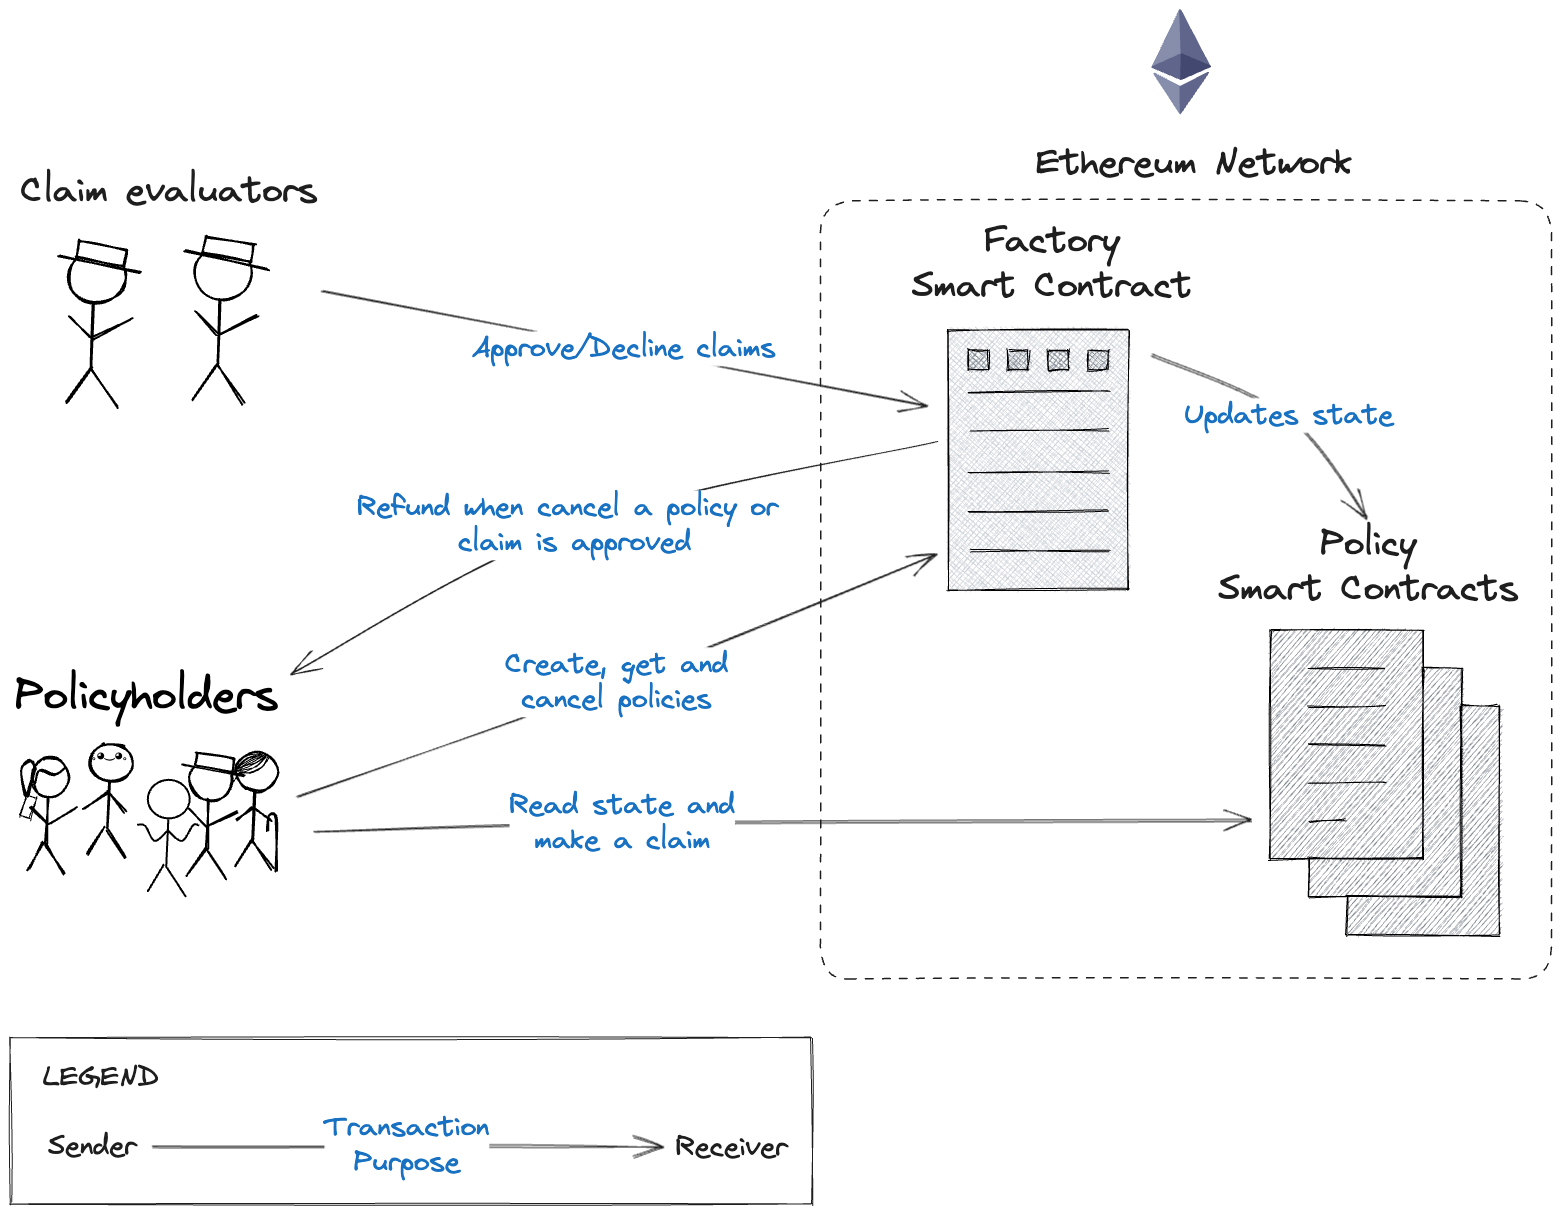
\includegraphics[width=14cm]{img/project-development/factory-policy.png}
\caption[Factory and policy smart contracts transaction flow]{\footnotesize{Factory and policy smart contracts transaction flow}}
\label{fig:smart-contracts-flow}
\end{figure}

The entire code of the Factory smart contract can be found in appendix \ref{appendix:factory-sc}.
}
\subsubsection{Ethereum developer environment}
{
To develop and test smart contracts a developer uses what is well-known as \textbf{testnet}, short for test network. The primary public network is called \textbf{Mainnet} and testing smart contracts here would imply consuming Mainnet \acrshort{eth} on transactions, which requires real money. Therefore, testnets are really useful to test potential smart contracts in a production-like environment before deployment to Mainnet, so it is the analogy to production and staging servers. For the experiment, there were two possibilities:
\begin{itemize}
    \item Use a local testnet, which requires selecting a feature that simulates the Ethereum network locally.
    \item Use a public testnet, which requires asking for testnet \acrshort{eth} to ``faucet entities", which distribute it sometimes free but with daily limitations. 
\end{itemize}

Since the public testnet option requires external dependencies to obtain \acrshort{eth} and the process can be challenging, I decided to use a local testnet through the tool \textbf{Hardhat}.

Hardhat is a tool that lets developers easily deploy contracts, run tests and debut Solidity code without dealing with live environments. Hardhat comes out-of-the-box with \textbf{Hardhat Network}\cite{hardhat_network}. It basically runs a process that implements the \acrshort{evm} and serves JSON-RPC and WebSocket requests. Moreover, it mines a block with each transaction that it receives so this really streamlines the developer experience. On server launch, it provides accounts with the public-private key pairs and a balance of 10.000 Hardhat \acrshort{eth}.

\begin{figure}[H]
\centering
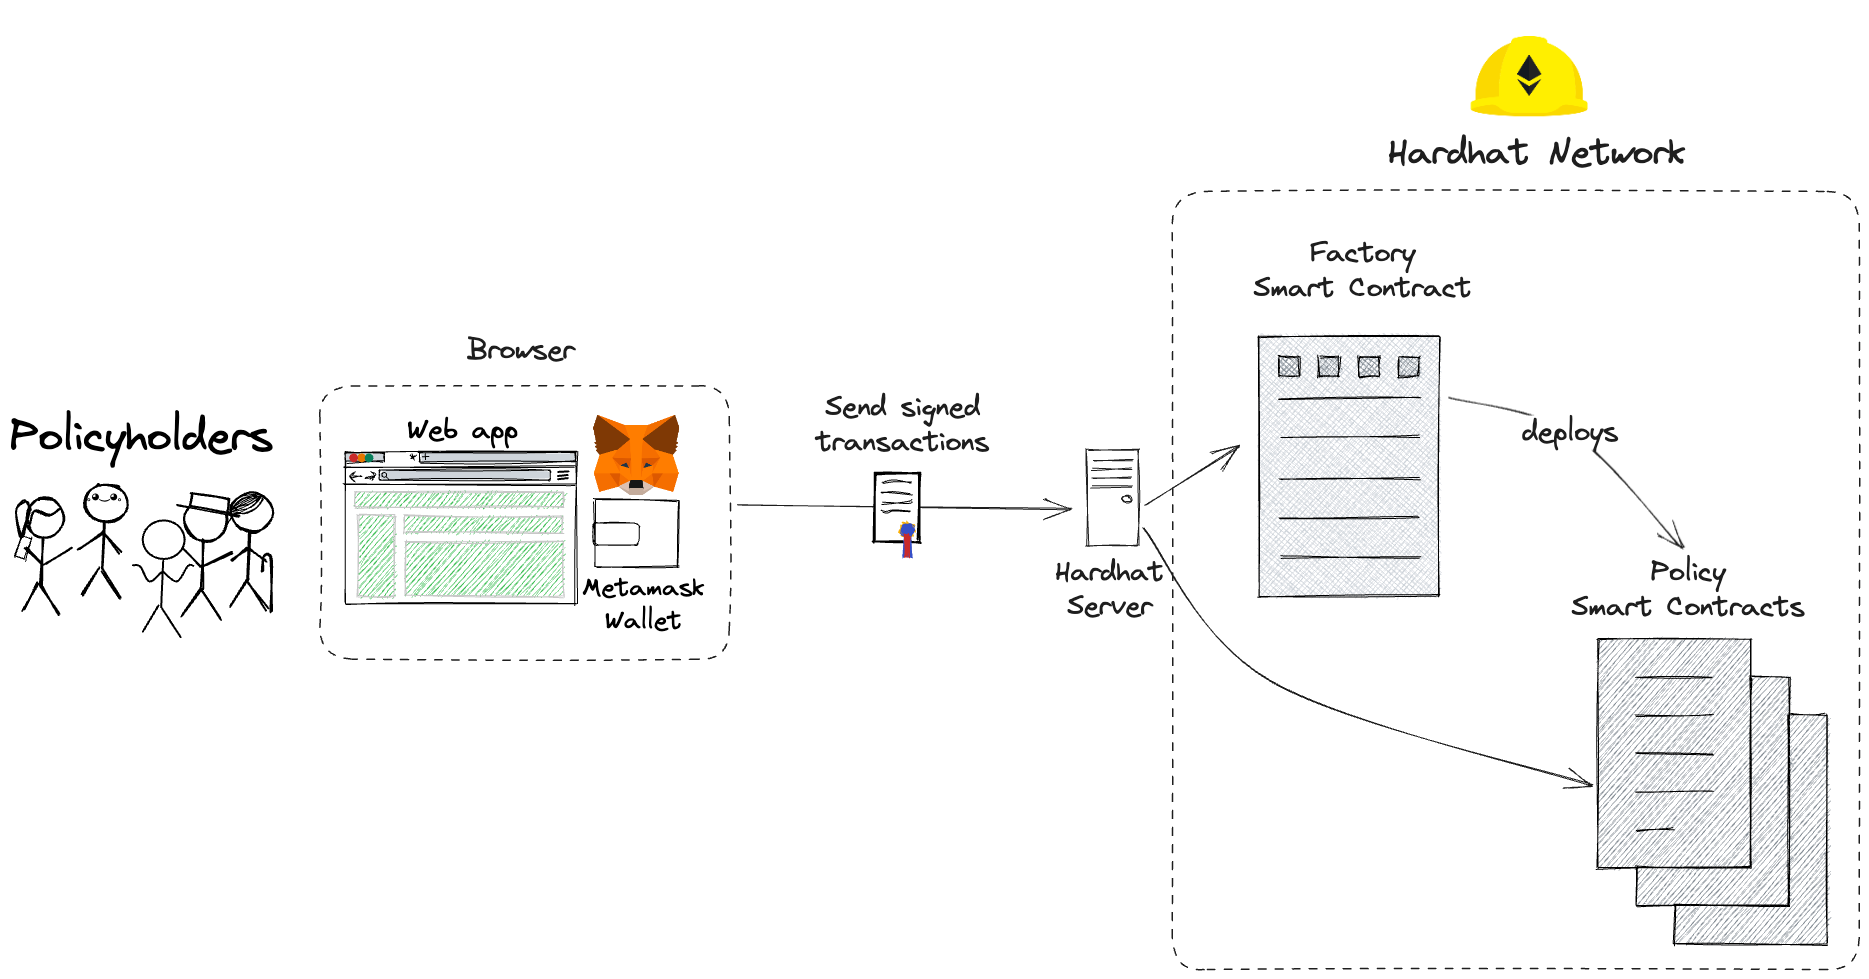
\includegraphics[width=14cm]{img/project-development/hardhat.png}
\caption[Web app consuming Hardhat network]{\footnotesize{Web app consuming Hardhat network}}
\label{fig:hardhat-network}
\end{figure}

In the experiment, the Hardhat network is served at a certain port, where the dapp will deploy the smart contract factory first, and then store the address of such contract into the web app application to make it accessible. As you may observe in figure \ref{fig:hardhat-network}, the web app and the Metamask wallet are configured to reach the factory smart contract and at this point, we are able to request transactions. 

The wallet is in charge of asking for user confirmation on each transaction, so they reach the network signed with the policyholder address. Note that every policy contract deployed through the factory creation process will be in the Hardhat network as well, so they are reachable by the web app too. 

}

\subsubsection{Security consideration}
{
There is an important security issue in this system. The data stored in the smart contracts is public so if it contains sensitive data anyone can see it. We can protect data making private or the getters with modifiers as explained above although, the miners can see all data in the nodes anyway. For our experiment, it does not represent an inconvenience but for a real case this problem could be solved by storing the data encrypted, for example using the public key of the user account to encrypt and the private key to decrypt. This is just a need to protect sensitive data but not necessary for changing the state since function executions can be protected, for instance by the address of the transaction sender.
}


\subsection{Off-blockchain backend}
{
The off-blockchain application consists of a backend app that handles proposal generation by providing pricing and storage of such proposals. There are many possible solutions to implement these requirements but the one selected for me is \textbf{NestJS}\cite{nestjs}.

NestJS is a framework for building efficient, scalable Node.js server-side applications. It is developed with Javascript\cite{javascript} and provides an out-of-the-box application architecture that allows developers to create highly testable, scalable, loosely coupled and easily maintainable applications.

Usually, a backend uses an \textit{\Gls{orm}}, Object-Relational mapping, which provides a way of mapping the data schemas with the backend models and eases the connection and comprehension. For the experiment, I selected \textbf{Prisma}, a new kind of \Gls{orm} which apart from offering really comprehensive documentation and easy implementation with NestJS, recently has grown in popularity because of the way it declares just a data schema as a single source of truth and generates the database and backend types according to this agreement. For the experiment, a \textbf{PostgreSQL}\cite{postgresql} database has been selected, which is a powerful, open-source object-relational database more than enough for storing some proposals.

Thanks to these technologies, I was able to implement the two expected features.

\subsubsection{Proposals module}
{
The goal of the module is to offer insurance coverage and the corresponding price given a specific car and driver data.
In addition, when the user likes the proposal he can save it to purchase it later on. To achieve this the app accepts several requests:
\begin{enumerate}
    \item The first request is through the endpoint \textbf{POST ``/api/proposals/quote"}. The body of this request basically consists of a risk subject and a risk object. The risk subject contains the driver data such as name, document number, and birth date, whilst the risk object collects all detailed specifications about the car. Just a few of this data has been required in favor of the real scenario. Some of these fields are maker and model, plate, fuel type, etc. The response contains the list of coverage services available with their monthly price respectively. 
    \item Once the request wants to be saved, the app offers the endpoint \textbf{POST ``/api/proposals/quote/save"}. The body for this case collects the same attributes as before, risk subject and risk object, but also the coverage configuration the user wants to include on his policy. 
   \item When a user wants to retrieve his saved proposals he can use the endpoint \textbf{GET ``/api/proposals/quote"}. To develop this feature the authentication module has to be implemented, which is explained in the section \ref{section:authentication-module}.
\end{enumerate}

With the previous endpoints, we enable the web app to ask for the data from the user and request the backend for a quote pricing. Once the backend responds, the coverage possibilities may be displayed to the user who then selects the coverage services that he would like to include. Eventually, if the proposal sounds good to him, he could save the proposal. The following step was to implement the authentication module to bind the proposals to the clients.
}

\subsubsection{Authentication module}
\label{section:authentication-module}
{
The authentication flow proposed for the dapp is a little bit different from the standard models since it uses the client wallets instead of a social media login or the usual email/password combination to identify a user.

Since we are using blockchain and we can assume each of our clients has an address, we can leverage these authentication credentials to identify them in our backend. The concept is called \textbf{nonce-based authentication} and is quite simple:
\begin{enumerate}
    \item A user wants to be authenticated so he asks the backend to generate a \gls{nonce}. The backend app generates the nonce and stores it for some time. Theoretically, this nonce cannot be generated again so each time is requested the app generates a different one. To generate this nonce it was used the library \textit{Siwe, Sign in with Ethereum}\cite{how-siwe}.
    \item Then, the user receives the nonce and signs it using his private key. Once signed he sends to backend the signed message along with the public key.
    \item Backend verifies that the message has been signed with the public key received and it contains the nonce provided previously, so it guarantees that the sender is the owner of the private key, the unique capable of signing the message, hence it is authenticated. The nonce gets removed from the backend storage and a token for authenticating the account is returned to the user in order to attach it to the headers and access protected endpoints.
\end{enumerate}
This behavior is achieved with two endpoints: \textbf{GET ``/api/auth/generate-nonce"} and \textbf{POST ``/api/auth/authenticate"} as you may observe in figure \ref{fig:auth-flow}. At this point, the backend app can protect the endpoint for saving proposals, so the proposals will be always sent with an authentication header including the token that identifies the user and we can bind the proposal to him.

\begin{figure}[H]
\centering
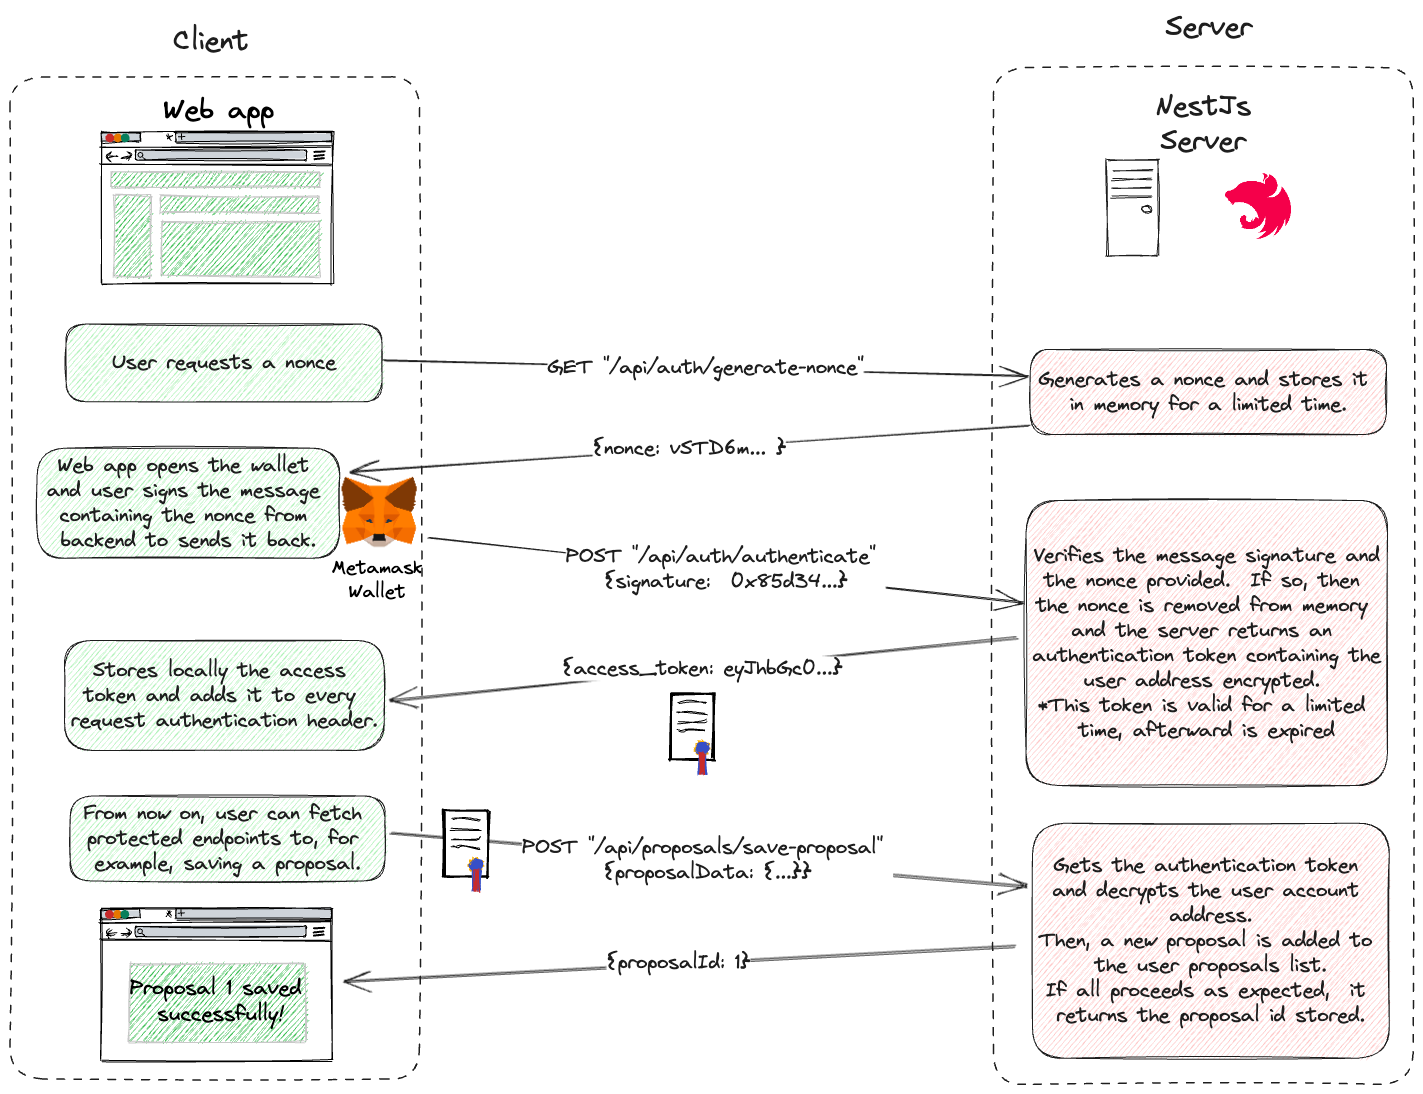
\includegraphics[width=14cm]{img/project-development/nonce.png}
\caption[Authentication flow]{\footnotesize{Authentication flow}}
\label{fig:auth-flow}
\end{figure}

In addition, the endpoint to get user proposals must be protected as well so it requires the authentication token. Therefore, when the backend app receives a request, it checks the token, gets the account and retrieves the list of proposals for that user. This idea of authenticating through the Ethereum account is based on the articles \cite{how-siwe} and \cite{why-siwe}.

}
}

\subsection{Frontend}
{
The frontend app is the last piece to complete the system. It aims to provide a platform for the users that want to interact with the dapp. Moreover, it will be the unique software to interact with both, off-blockhain and on-blockchain backends.

There are many technologies to develop a frontend web application. For the experiment, I selected \textbf{Next.js}. Next.js is a \textbf{React}\cite{reactjs} framework to create full-stack web applications that include out-of-the-box features to compile, bundle and build the application which reduces widely the time spent in configuration. This is one of the most common solutions adopted by the frontend community.

React, like most of the libraries to develop web applications, is based on the idea of building User Interface (UI) components and composing them like a tree with nodes in the DOM in order to eventually create interactive pages as is represented in the figure \ref{fig:react-dom}. Such components can be compared to math functions, which receive input data and return visual elements that are displayed in the browser. 

In addition, components can pass data to other components and react to user interactions such as clicking a button or filling out a form. Every event or change triggers a render which means the component is computed again to display the change in the layout and it propogates the change to the child components. React counts on a really efficient algorithm called ``\textit{Virtual DOM}" to compute the changes between two renders and display the new UI immediately in the browser \Gls{dom}. 

\begin{figure}[H]
\centering
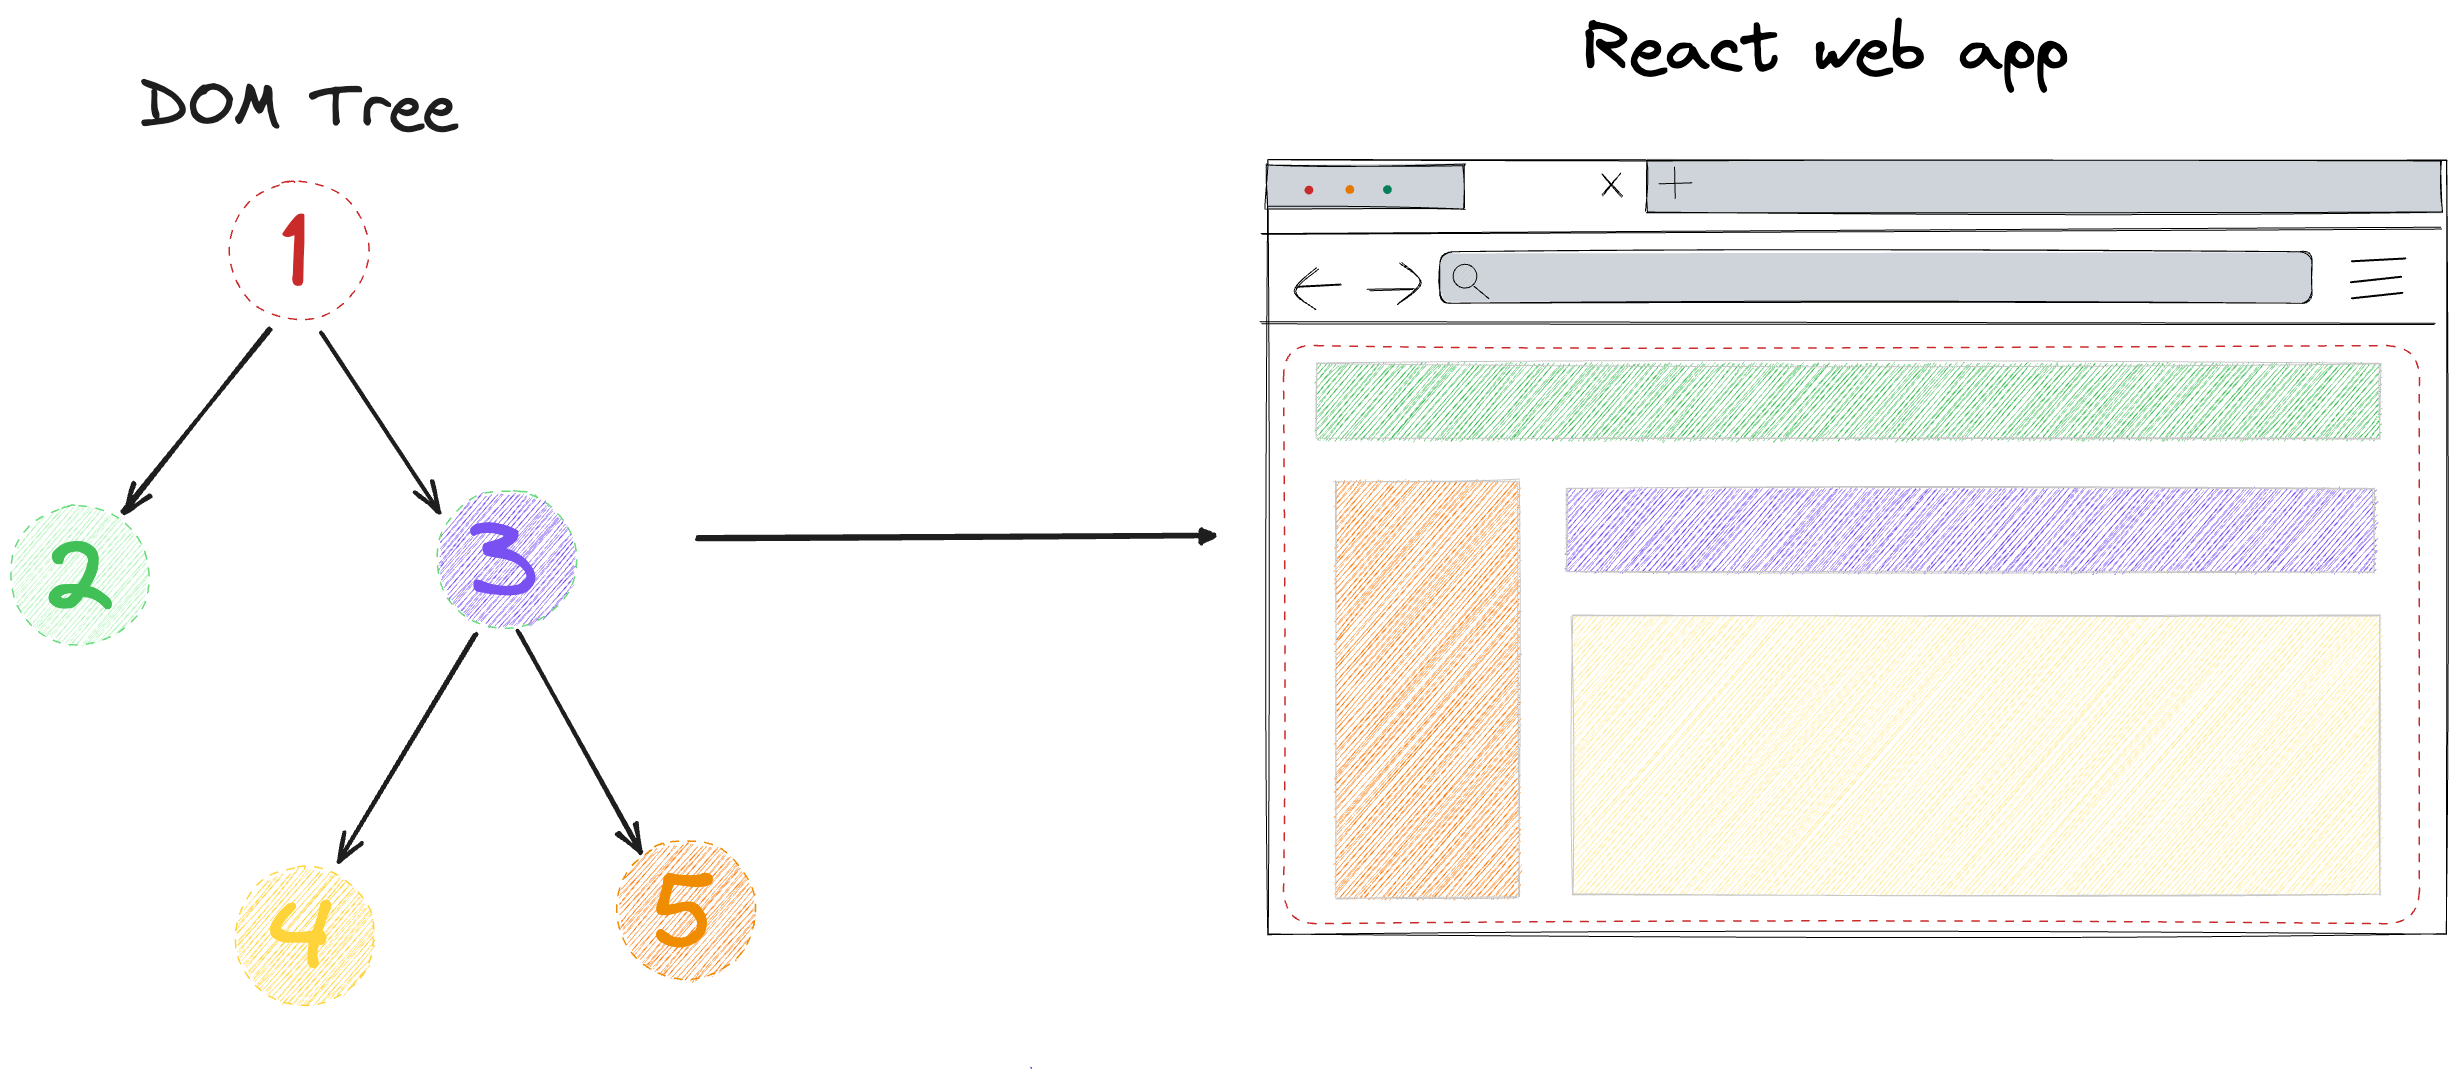
\includegraphics[width=14cm]{img/project-development/react-dom.png}
\caption[React tree to browser DOM]{\footnotesize{React tree to browser DOM.}}
\label{fig:react-dom}
\end{figure}

Next.js provides a powerful layer which is known as \textbf{Server side rendering (SSR)}. As you may see in figure \ref{fig:ssr}, when the user requests a web page SSR server pre-renders the content in the server and responds with the first version rendered to the client. This significantly enhances the user first-load experience and page indexation in browser engines. Once the app is displayed on the client, the next renders happen on the client side. 

\begin{figure}[H]
\centering
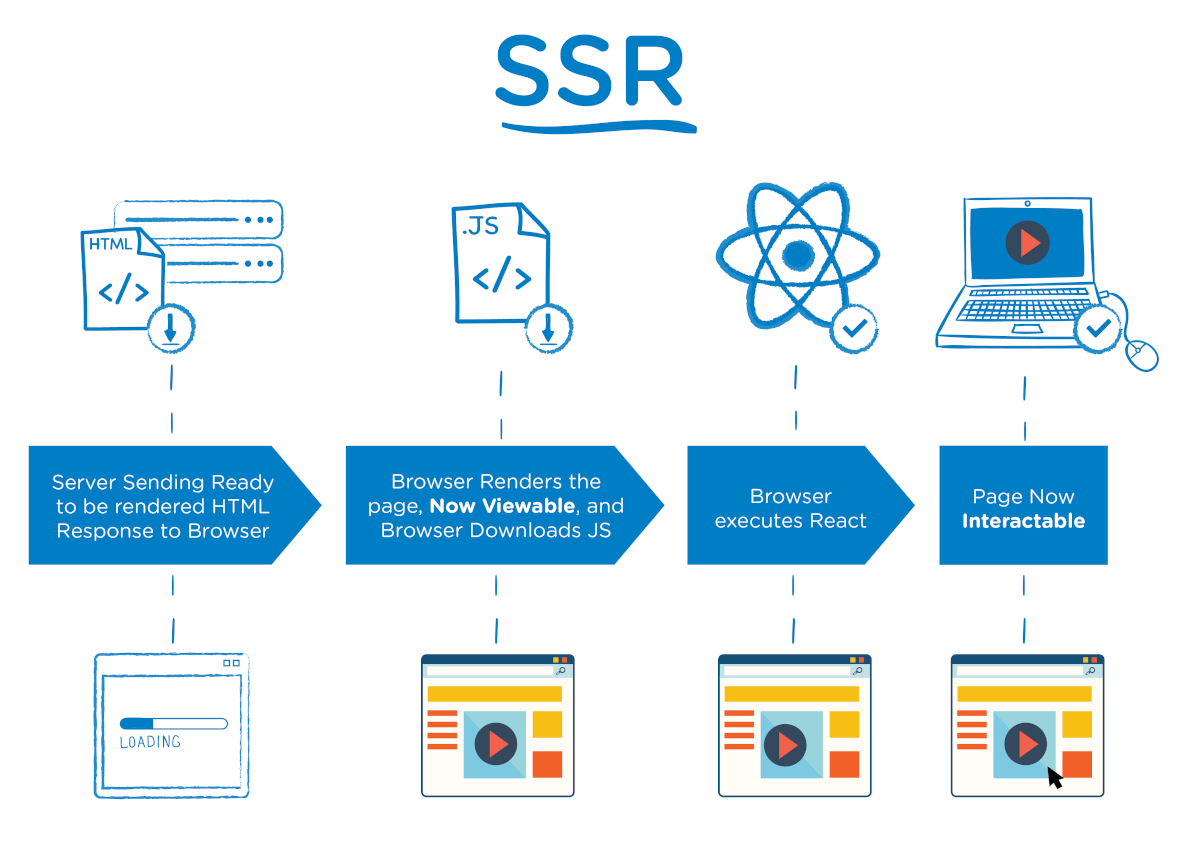
\includegraphics[width=14cm]{img/project-development/ssr.png}
\caption[Server side rendering of web applications]{\footnotesize{Server side rendering of web applications.}}
\label{fig:ssr}
\end{figure}

The project has used libraries like \textit{Material UI}\cite{mui}, which provide a huge amount of stylish and pretty components that can be used to ease the design and development process resulting in a more fancy layout. About the blockchain part, it consumes the ABI's generated by the contracts compilation and along with the Javascript libraries \textit{wagmi.sh} and \textit{ethers.js}\cite{ethers}, the communication with the smart contracts and the wallet becomes pretty straightforward.
}


\subsection{Version control}
{
All the code of the project has been stored in \textbf{Github}\cite{github}, a cloud version control storage that allows us to host our \textbf{Git} repository. Git\cite{git} is an open-source version control system worldwide used by developers to work with code in a traceable, organized, and clean way. It lets the developers access all the codebase history, creating incremental versions and forking to try different ideas but also merge when necessary.

Having all the code centralized in a single source of truth, which let me create different versions or approaches of the experiment was fundamental to not blocking the progress of the project and working on several features without breaking a stable incremental version.
}